\section{Aufgabe 4 - Wertbestimmung von Widerstand und Kondensator}
\label{sec:aufgabe-4---wertbestimmung-von-widerstand-und-kondensator}

In dieser Aufgabe geht es um Widerstände und Kondensatoren.
Diese sind Grundbausteine der Elektrotechnik.
Neben diversen Berechnungen sind folgende Fragen zu beantworten.

\begin{itemize}
    \item Können Unterschiede zwischen Messungen am Mikrocontroller und manuellen Methoden gefunden werden?
    \item Wenn Ja, welche und warum?
    \item Mit welchen Prinzipien und Überlegungen wurden die Widerstände gemessen?
    \item Welche Abweichungen ergeben sich beim Messen bekannter Kondensatoren?
\end{itemize}

\subsection{Materialien}
\label{subsec:a4-materialien}

\begin{table}[h]
    \centering
    \caption{Aufgabe 4 - Verwendete Materialien}
    \label{tab:a4-materialien}
    \begin{tabular}{| l | l | l |}
        \hline
        Bezeichnung & Eigenschaften & Menge \\
        \hline
        Widerstand  & $10k\Omega$   & 2     \\
        & Braun - Schwarz - Orange - Gold & \\
        Widerstand & unbekannt & k.A. \\
        Mikrocontroller & Arduino Uno R3 & 1 \\
        \hline
    \end{tabular}
\end{table}

In der Tabelle \ref{tab:a4-materialien} sind unbekannte Widerstände in nicht angegebener Menge gelistet.
Damit sind Testwiderstände gemeint, welche durch das Testen an der Schaltung gemessen werden können.
Beim Versuch an dieser Schaltung sind die Widerstandswerte normalerweise bekannt, um die Richtigkeit der Schaltung zu bestätigen.
Die Werte und Anzahl der verwendeten Widerstände sind jedoch nicht relevant.

\subsection{Vorbereitung}
\label{subsec:a4-vorbereitung}

\subsubsection{Aufgabe 1}

In dieser Aufgabe sind Widerstände an Hand ihrer Farbcodes zu bestimmen.
Drei Widerstände sind gegeben.
Anhand der Tabelle in Sektion \ref{tab:farbcodierung-von-widerständen} kann der Wert bestimmt werden.

\begin{table}[ht]
    \centering
    \caption{Widerstandswerte}
    \label{tab:a4-widerstandswerte}
    \begin{tabular}{| l | l | l | l | l | l |}
        \hline
        Ring 1 & Ring 2 & Ring 3 & Ring 4 & Widerstandswert & Toleranz \\
        \hline
        Gelb & Violett & Rot & Gold & $4,7k\Omega$ & $\pm5\%$ \\
        Rot & Weiß & Grün & Gold & $3,9M\Omega$ & $\pm5\%$ \\
        Blau & Grau & Rot & Silber & $6,8k\Omega$ & $\pm10\%$ \\
        \hline
    \end{tabular}
\end{table}

\subsubsection{Aufgabe 2}

In Aufgabe 2 ist die Schaltung aus Abbildung \ref{fig:schaltung-a4-2} gegeben.

\begin{figure}[ht]
    \centering
    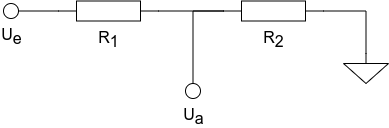
\includegraphics[width=\textwidth]{pictures/a4-1.png}
    \caption{Schaltung aus der Angabe aus Aufgabe 4.2}
    \label{fig:schaltung-a4-2}
\end{figure}

Für den ersten Teil sind folgende Werte gegeben.
\begin{itemize}
    \item $U_e = 5V$
    \item $U_a = 3V$
\end{itemize}

Nun soll ermittelt werden, welches Verhältnis zwischen den Widerständen $R_1$ und $R_2$ herrschen muss, damit der gegeben Zustand möglich ist.
Um den Spannungsabfall über einen Widerstand zu ermitteln, kann die Formel des Spannungsteilers verwendet werden.

\begin{align}
    U_R = \frac{U}{R_{ges}} * R
\end{align}

Unter berücksichtigung der Angaben können die Werte eingesetzt werden.

\begin{align}
    U_a = \frac{U_e}{R_1 + R_2} * R_2
\end{align}

Nun kann umgeformt werden, um ein Verhältnis zwischen $R_2$ und $R_{ges}$ zu erhalten.

\begin{align}
    U_a = \frac{U_e}{R_1 + R_2} * R_2 \Rightarrow\\
    \frac{U_a}{U_e} = \frac{R_2}{R_{ges}} \Rightarrow\\
    \frac{3}{5} = \frac{R_2}{R_{ges}}
\end{align}

Daher gilt:

\begin{align}
    \frac{3}{5} = \frac{R_2}{R_{ges}} \Rightarrow \frac{2}{5} = \frac{R_1}{R_{ges}} \Rightarrow \\
    \frac{3}{5} * R_{ges} = R_2 \text{ und } \frac{2}{5} * R_{ges} = R_1 \Rightarrow
\end{align}

Das Verhältnis zwischen den Widerständen kann nun berechnet werden.

\begin{align}
    \frac{R_1}{R_2} = \\
    \frac{\frac{2}{5} * \cancel{R_{ges}}}{\frac{3}{5} * \cancel{R_{ges}}} = \\
    \frac{\frac{2}{\cancel{5}}}{\frac{3}{\cancel{5}}} = \\
    \frac{2}{3}
\end{align}

Nun muss berechnet werden, wie hoch der Widerstand $R_2$ sein muss, wenn $R_1 = 10k\Omega$ gilt.

\begin{align}
    (10) \land (13) \Rightarrow \\
    \frac{R_1}{R_2} = \frac{2}{3} \Rightarrow \\
    \frac{3 * 10k\Omega}{2} = R_2 = 15k\Omega
\end{align}

Nun soll ein unbekannter Widerstand $R_x$ berechnet werden, wenn $R_1 = 10k\Omega$ und $U_a = 1V$ gilt.
Für den Spannungsteiler gilt nun folgendes.

\begin{align}
    U_a = \frac{U_e}{R_x + R_1} * R_x \Rightarrow \\
    U_e = \frac{U_a * (R_x + R_1)}{R_x} \Rightarrow \\
    \frac{U_e}{U_a} = \frac{R_x}{R_x} + \frac{R_1}{R_x} \Rightarrow \\
    \frac{U_e}{U_a} - 1 = \frac{R_1}{R_x} \Rightarrow \\
    R_x = \frac{R_1}{\frac{U_e}{U_a} - 1} \Rightarrow \\
    R_x = \frac{R_1}{\frac{U_e - U_a}{U_a}} \Rightarrow\\
    R_x = \frac{\frac{R_1 * U_a}{U_a}}{\frac{U_e - U_a}{U_a}} \Rightarrow \\
    R_x = \frac{R_1 * U_a}{U_e - U_a}
\end{align}

Durch einsetzen der gegebenen Werte ergibt sich nun ein Wert für $R_x$.

\begin{align}
    (24) => \\
    R_x = \frac{R_1 * U_a}{U_e - U_a} = \\
    \frac{10k\Omega * 1V}{5V - 1V} = \\
    \frac{10k\Omega V}{4V} \Rightarrow \\
    R_x = 2,5k\Omega
\end{align}

\subsubsection{Aufgabe 3}

In dieser Aufgabe wird ein Kondensator über einen Wiederstand $R = 10k\Omega$ an einer Spannungsquelle $U_q$ geladen.
Die Spannung des Kondensators ist $U_c(0) = 0V$ und $U_c(0,1s) = 0,63 * U_q$.
Es soll die Kapazität des Kondensators ermittelt werden.

Die Formel zur Berechnung der Spannung des Kondensators lautet folgendermaßen.

\begin{align}
    U_c(t) = \frac{1}{C} * I * t
\end{align}

Dies kann folgendermaßen umgeformt werden.

\begin{align}
    U_c(t) = \frac{1}{C} * I * t = \\
    \frac{1}{C} * \frac{U_q}{R} * t \Rightarrow \\
    C = \frac{U_c(t)}{\frac{U_q}{R} * t}
\end{align}

Nun können die Werte der Angabe eingesetzt werden.

\begin{align}
    (33) \Rightarrow \\
    C = \frac{0,63 * U_q}{\frac{U_q}{10k\Omega} * 0,1s} = \\
    \frac{0,63}{\frac{1}{10k\Omega} * 0,1s} = \\
    15\mu F
\end{align}

Nun soll ermittelt werden, wie lange es dauert, denn Kondensator vollständig zu laden.
Wir wissen:

\begin{align}
    \tau = RC \Rightarrow \\
    \tau = 0,15s
\end{align}

Weiters ist bekannt

\begin{align}
    U_c \geq 0,99U_Q \Leftrightarrow \text{nach } 5\tau
\end{align}

daraus folgt

\begin{align}
    t_{99\%} = 5\tau = 0,75s
\end{align}
\subsection{Praktikumsaufgabe}
\label{subsec:a4-praktikumsaufgabe2}

Es wurde die in Abbildung \ref{fig:a4-1-implemtierung} gezeigte Schaltung implementiert.
Am Steckbrett ist eine ähnliche Schaltung wie in Abbildung \ref{fig:schaltung-a4-2} zu sehen.
Der Pin A0 ist zwischen den bekannten $10k\Omega$ und den unbekannten Widerstand geschaltet.
Nun sind folgende WGrößen bekannt.

\begin{itemize}
    \item $V_{out}$ des Mikrocontrollers $V_{out} = 5V$
    \item Der bekannte Widerstand zwischen $V_{out}$ und A0, $R_1 = 10k\Omega$
\end{itemize}

Durch die Überlegung von (26) kann im Mirocontroller ein Programm implementiert werden, welches den unbekannten Widerstand errechnet.

\begin{figure}[ht]
\centering
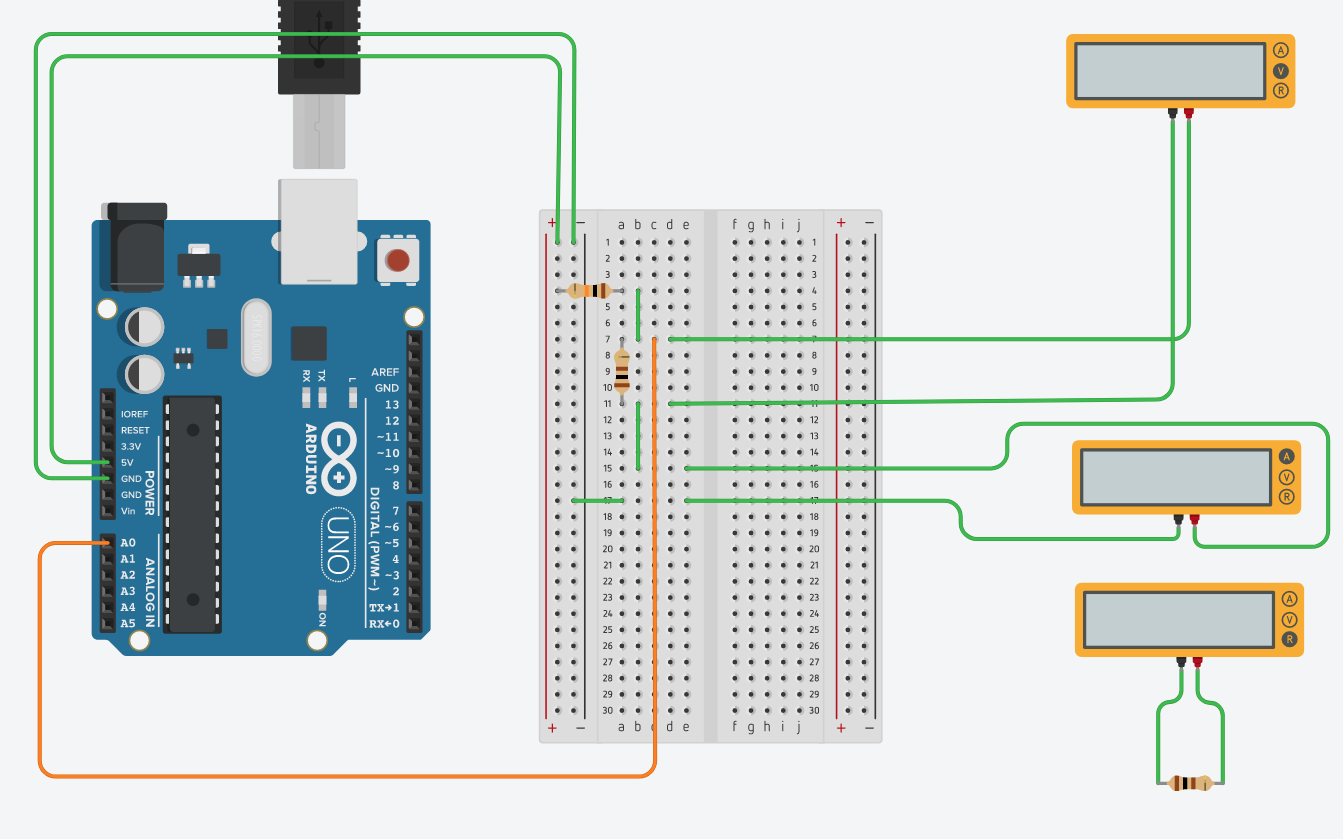
\includegraphics[width=\textwidth]{pictures/a4-1-praktik.png}
\caption{Implementierter Stromkreis von Aufgabe 4.1}
\label{fig:a4-1-implemtierung}
\end{figure}

Im nachfolgendem Text wird der Programmcode der Aufgabe erläutert.
Einzelne Teile des Codes werden ausgewählt und beschrieben.
Am Ende dieser Sektion befindet sich der vollständige Programmcode.

\begin{lstlisting}[language=C,label={lst:a4-1-konstanten}, caption={Konstanten der Aufgabe 4.1}]
const int PIN_VOLTAGE = A0;
const float U_IN = 5;
const float RESOLUTION = U_IN / 1024;
const int RESISTOR = 10 * 1000;
\end{lstlisting}

Durch den Code in Listing \ref{lst:a4-1-konstanten} werden die bekannten Größen angelegt.
\textit{U\_IN} gibt die Spannung in Volt an, während \textit{RESISTOR} den Widerstandswert abbildet.
Die Konstante \textit{RESOLUTION} bedarf genauerer Erklärung.

Die analogen Pins des Microkontroller können Spannungen zwischen 0V und 5V auslesen.
Um diese als Zahl darzustellen, wird ein Wert zwischen 0 und 1024 zurückgegeben.
Hierbei steht 0 für 0V und 1024 für 5V.
Das Interval $(0V, 5V)$ wird daher auf das Interval $(0, 1024)$ abgebildet.
Um die Spannung nun in Volt zu erhalten, muss mit der Wert aus A0 mit $\frac{5V}{1024}$ multipliziert werden.
Dieser Multiplikator wird in der Konstante \textit{RESOLUTION} gespeichert.

Der verwendete Microkontroller konfiguriert analoge Pins standardmäßig als Input-Pins.
Eine explizite Konfiguration als solche in der $setup()$ Funktion ist also nicht notwendig.

\begin{lstlisting}[language=C,label={lst:a4-1-loop}, caption={Programmschleife der Aufgabe 4.1}]
void loop()
{
    int value = analogRead(PIN_VOLTAGE);
    float u_a = value * RESOLUTION;
    float r = (u_a * RESISTOR) / (U_IN - u_a);

    Serial.println("");
    Serial.print(u_a);
    Serial.println(" V");
    Serial.print(r);
    Serial.println(" Ohm");
    delay(1000);
}
\end{lstlisting}

In Listing \ref{lst:a4-1-loop} wird zuerst der derzeitige Wert des Pins A0 ausgelesen und in der variable \textit{value} abgelegt.
Dieser Wert wird nun mit den in Listing \ref{lst:a4-1-konstanten} angelegten Multiplikator \textit{RESOLUTION} multipliziert, um die Spannung $U_a$, vergleiche \ref{fig:stromkreis-a1}, zu erhalten.
Durch die Überlegung aus (26) kann nun der Widerstand $R_2$, bzw. $R_x$, errechnet werden.

Danach erfolgt die Ausgabe über der errechneten Größen über die serielle Schnittstelle.
Ein Pausieren des Programms wird durchgeführt, um ein angenehmeres Lesen der Ausgabe zu ermöglichen.

\begin{lstlisting}[language=C,label={lst:a4-1-programmcode}, caption={Vollständiger Programmcode der Aufgabe 4.1}]
const int PIN_VOLTAGE = A0;
const float U_IN = 5;
const float RESOLUTION = U_IN / 1024;
const int RESISTOR = 10 * 1000;

void setup()
{
    Serial.begin(9600);
}

void loop()
{
    int value = analogRead(PIN_VOLTAGE);
    float u_a = value * RESOLUTION;
    float r = (u_a * RESISTOR) / (U_IN - u_a);

    Serial.println("");
    Serial.print(u_a);
    Serial.println(" V");
    Serial.print(r);
    Serial.println(" Ohm");
    delay(1000);
}
\end{lstlisting}

\subsection{Fehlerdiskussion}
\label{subsec:a4-fehlerdiskussion}

\subsection{Zusammenfassung}
\label{subsec:a4-zusammenfassung2}
